\documentclass[12pt]{article}
\usepackage[english]{babel}
\usepackage[utf8]{inputenc}

%% Pointer to 'default' preamble
% pacakages and definitions

\usepackage{geometry}
\geometry{
	letterpaper, 
	portrait, 
	top=.75in,
	left=.8in,
	right=.75in,
	bottom=.5in		} 	% Page Margins
	
%% additional packages for nice things
\usepackage{amsmath} 	% for most math
\usepackage{commath} 	% for abs
\usepackage{lastpage}	% for page count
\usepackage{amssymb} 	% for therefore
\usepackage{graphicx} 	% for image handling
\usepackage{wrapfig} 	% wrap figures
\usepackage[none]{hyphenat} % for no hyphenations
\usepackage{array} 		% for >{} column characterisctis
\usepackage{physics} 	% for easier derivative \dv....
\usepackage{tikz} 		% for graphic@!
\usepackage{circuitikz} % for circuits!
\usetikzlibrary{arrows.meta} % for loads
\usepackage[thicklines]{cancel}	% for cancels
\usepackage{xcolor}		% for color cancels
\usepackage[per-mode=fraction]{siunitx} % for si units and num
\sisetup{group-separator = {,}, group-minimum-digits = 3} % additional si unit table functionality

\usepackage{fancyhdr} 	% for header
\usepackage{comment}	% for ability to comment out large sections
\usepackage{multicol}	% for multiple columns using multicols
\usepackage[framed,numbered]{matlab-prettifier} % matlab sytle listing
\usepackage{marvosym} 	% for boltsymbol lightning
\usepackage{pdflscape} 	% for various landscape pages in portrait docs.
%\usepackage{float}
\usepackage{fancyvrb}	% for Verbatim (a tab respecting verbatim)
\usepackage{enumitem}	% for [resume] functionality of enumerate
\usepackage{spreadtab} 	% for using formulas in tables}
\usepackage{numprint}	% for number format in spread tab
\usepackage{subcaption} % for subfigures with captions
\usepackage[normalem]{ulem} % for strike through sout

% for row colors in tables....
\usepackage{color, colortbl}
\definecolor{G1}{gray}{0.9}
\definecolor{G2}{rgb}{1,0.88,1}%{gray}{0.6}
\definecolor{G3}{rgb}{0.88,1,1}

% For table formatting
\usepackage{booktabs}
\renewcommand{\arraystretch}{1.2}
\usepackage{floatrow}
\floatsetup[table]{capposition=top} % put table captions on top of tables

% Caption formating footnotesize ~ 10 pt in a 12 pt document
\usepackage[font={small}]{caption}

%% package config 
\sisetup{output-exponent-marker=\ensuremath{\mathrm{E}}} % for engineer E
\renewcommand{\CancelColor}{\color{red}}	% for color cancels
\lstset{aboveskip=2pt,belowskip=2pt} % for more compact table
%\arraycolsep=1.4pt\def
\setlength{\parindent}{0cm} % Remove indentation from paragraphs
\setlength{\columnsep}{0.5cm}
\lstset{
	style      = Matlab-editor,
	basicstyle = \ttfamily\footnotesize, % if you want to use Courier - not really used?
}
\renewcommand*{\pd}[3][]{\ensuremath{\dfrac{\partial^{#1} #2}{\partial #3}}} % for larger pd fracs
\renewcommand{\real}[1]{\mathbb{R}\left\{ #1 \right\}}	% for REAL symbol
\newcommand{\imag}[1]{\mathbb{I}\left\{ #1 \right\}}	% for IMAG symbol
\definecolor{m}{rgb}{1,0,1}	% for MATLAB matching magenta
	
%% custom macros
\newcommand\numberthis{\addtocounter{equation}{1}\tag{\theequation}} % for simple \numberthis command

\newcommand{\equal}{=} % so circuitikz can have an = in the labels
\newcolumntype{L}[1]{>{\raggedright\let\newline\\\arraybackslash\hspace{0pt}}m{#1}}
\newcolumntype{C}[1]{>{\centering\let\newline\\\arraybackslash\hspace{0pt}}m{#1}}
\newcolumntype{R}[1]{>{\raggedleft\let\newline\\\arraybackslash\hspace{0pt}}m{#1}}

%% Header
\pagestyle{fancy} % for header stuffs
\fancyhf{}
% spacing
\headheight 29 pt
\headsep 6 pt

%% Header
\rhead{Thad Haines \\ Page \thepage\ of \pageref{LastPage}}
\chead{Mini WECC \\   10 Minute AGC Recovery (Generator Trips 01)}
\lhead{Research \\ 08/18/20}

\usepackage[hidelinks]{hyperref} % allow links in pdf
\usepackage{setspace}
\usepackage{multicol}
\usepackage{minted}

\begin{document}
\onehalfspacing
\paragraph{10 Minute AGC Recovery of Mini WECC after 2 Generator Trips} \ \\

\begin{minipage}{0.47\linewidth}
\begin{itemize}
\item Mini WECC system:
\begin{itemize}
\itemsep 0 em
\small
\item Buses: 122
\item Lines: 171
\item Loads: 88
\item Machines: 34
\item States: 623
\end{itemize}
\item Events: Trip of Bus 1 Gen at t= 5\\ Trip of Bus 30 Gen at t = 8

\item Each area has identical conditional AGC that acts at t=40 and again when t=160, 280, 400, 520 (i.e. 2 minute action time).

\item ODE solver tolerances:
\subitem Relative: 1e-5
\subitem Absolute: 1e-7

\end{itemize}
\vfill
\end{minipage}\hspace{2em}% 
\begin{minipage}{0.47\linewidth}
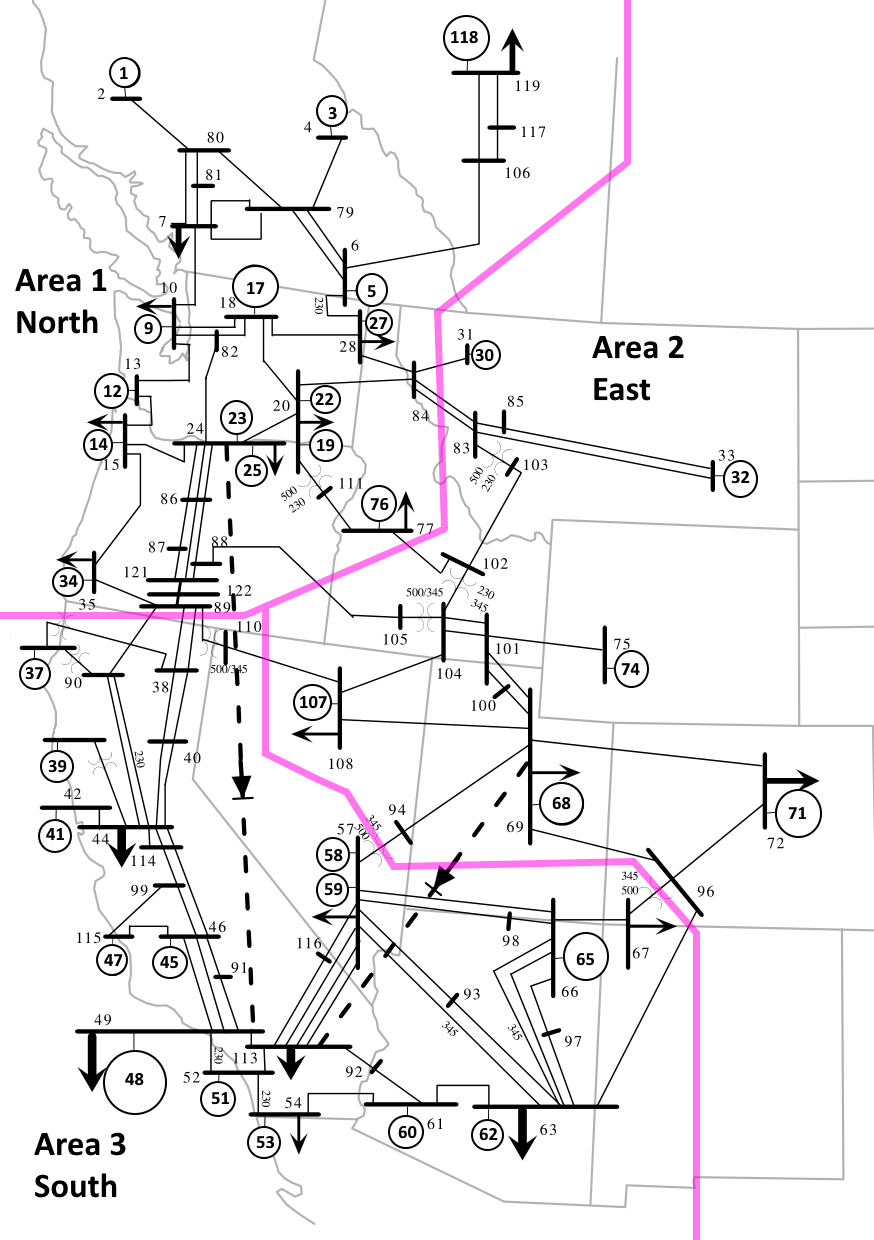
\includegraphics[width=.97\linewidth]{miniWECC_split03.png}
\end{minipage}% 

\paragraph{Result Summary:}
\begin{itemize}
\item Generators trip successfully, average system frequency and system inertia calculated correctly.
\item AGC controlled machines hit generation limits - Case needs minor adjustment.
\item Tripped generator states and derivatives affect size of time step.
\end{itemize}

\begin{center}
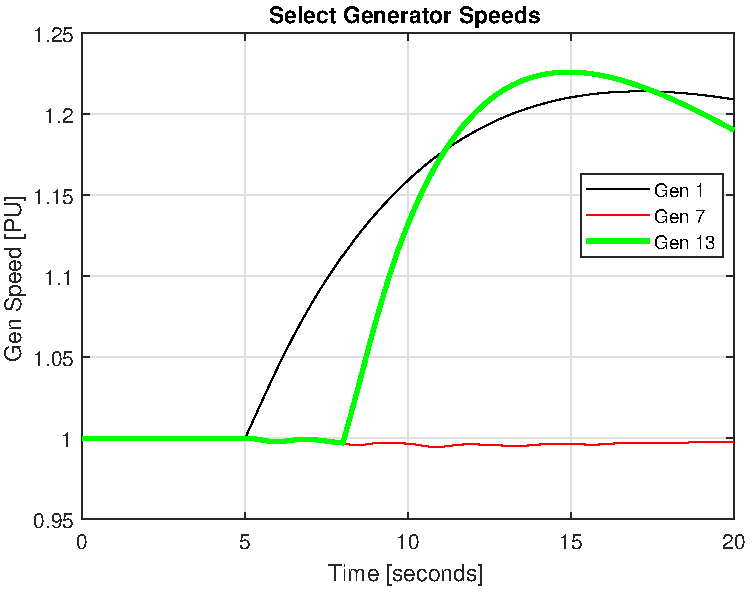
\includegraphics[width=.45\linewidth]{genTripSPD01}%
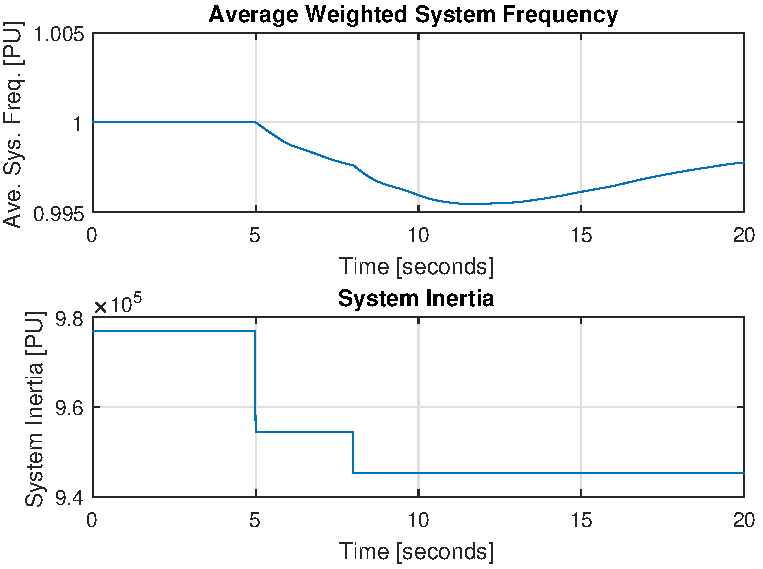
\includegraphics[width=.45\linewidth]{genTripFnH01}%
\end{center}


\pagebreak
\paragraph{Select Comparisons: t = 0:600 (full simulation)} \ \\
System frequency does not return to 1 as controlled machine generation limits are hit.
AGC distributed ACE (DACE) continues to accumulate.
Time step does not increase past 0.2 seconds.

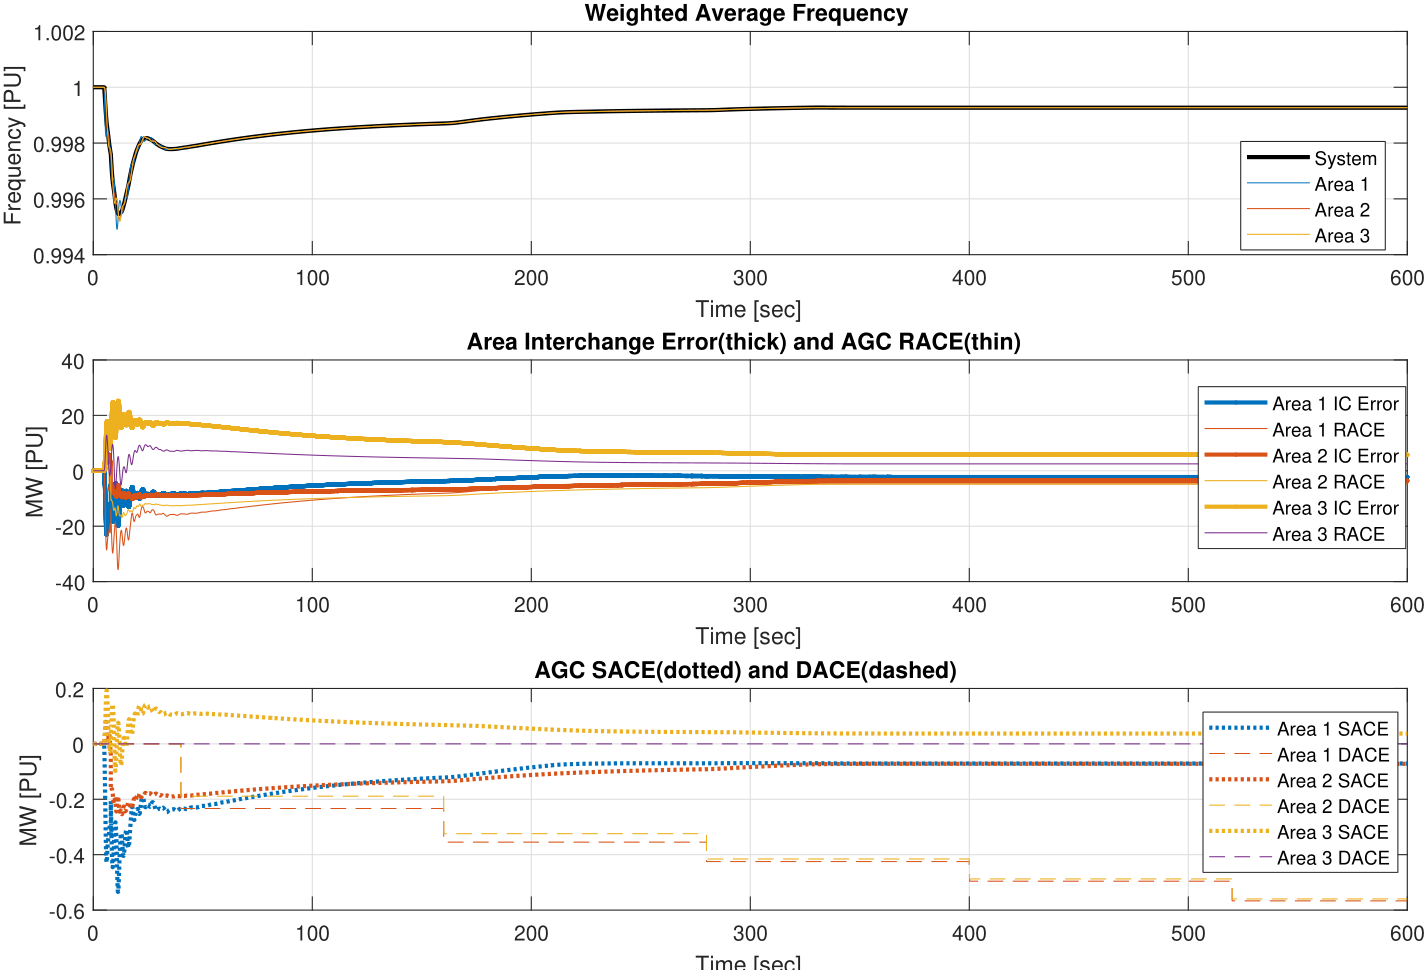
\includegraphics[width=\linewidth]{agc}


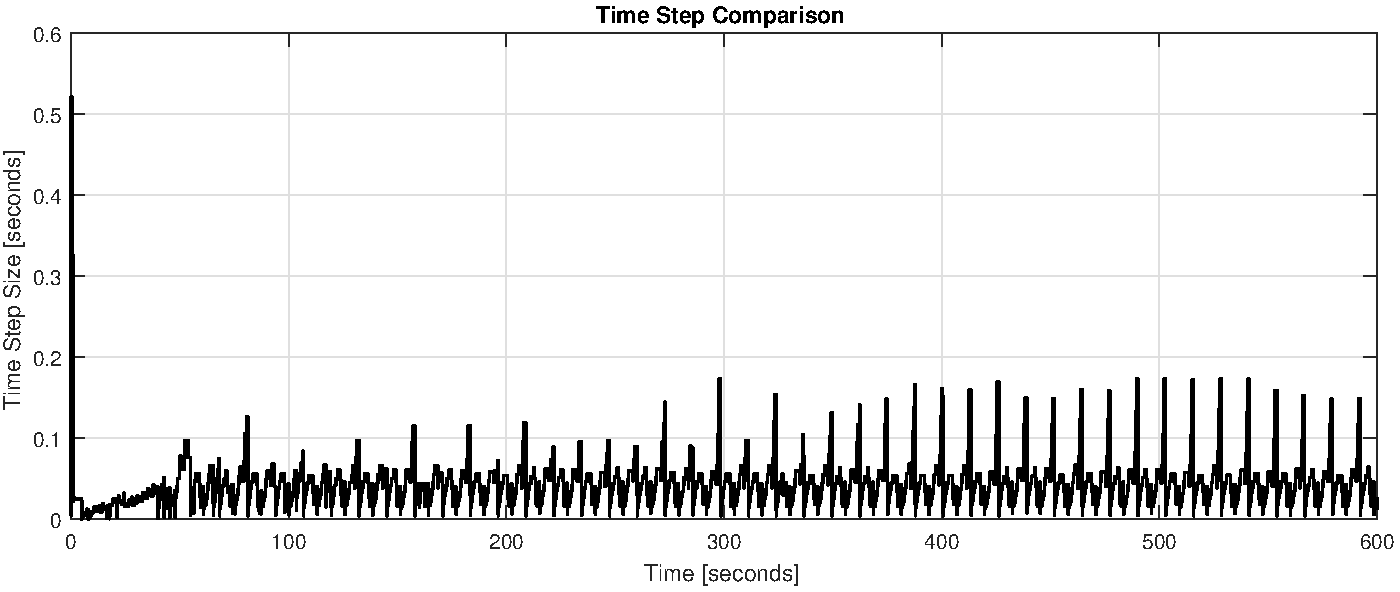
\includegraphics[width=\linewidth]{genTripteps01}

\pagebreak
\paragraph{EFD and Mechanical Power} \ \\
The oscillations of tripped generators affect the size of variable time steps as dynamic calculations still account for disconnected machines.
This is noticeable in exciter EFD and pmech oscillations of tripped generators.

\begin{center}
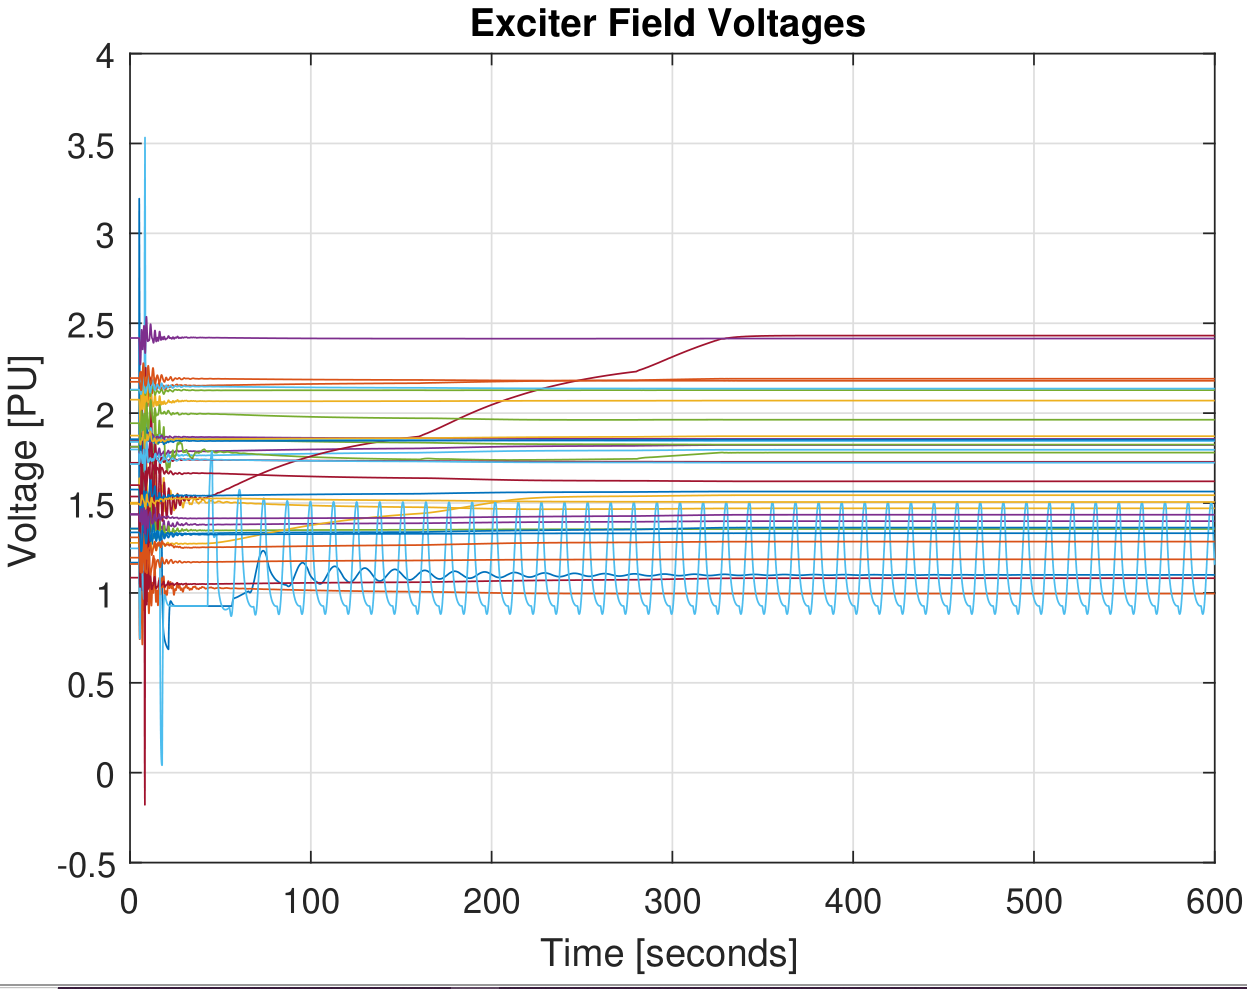
\includegraphics[width=.5\linewidth]{efd}% 
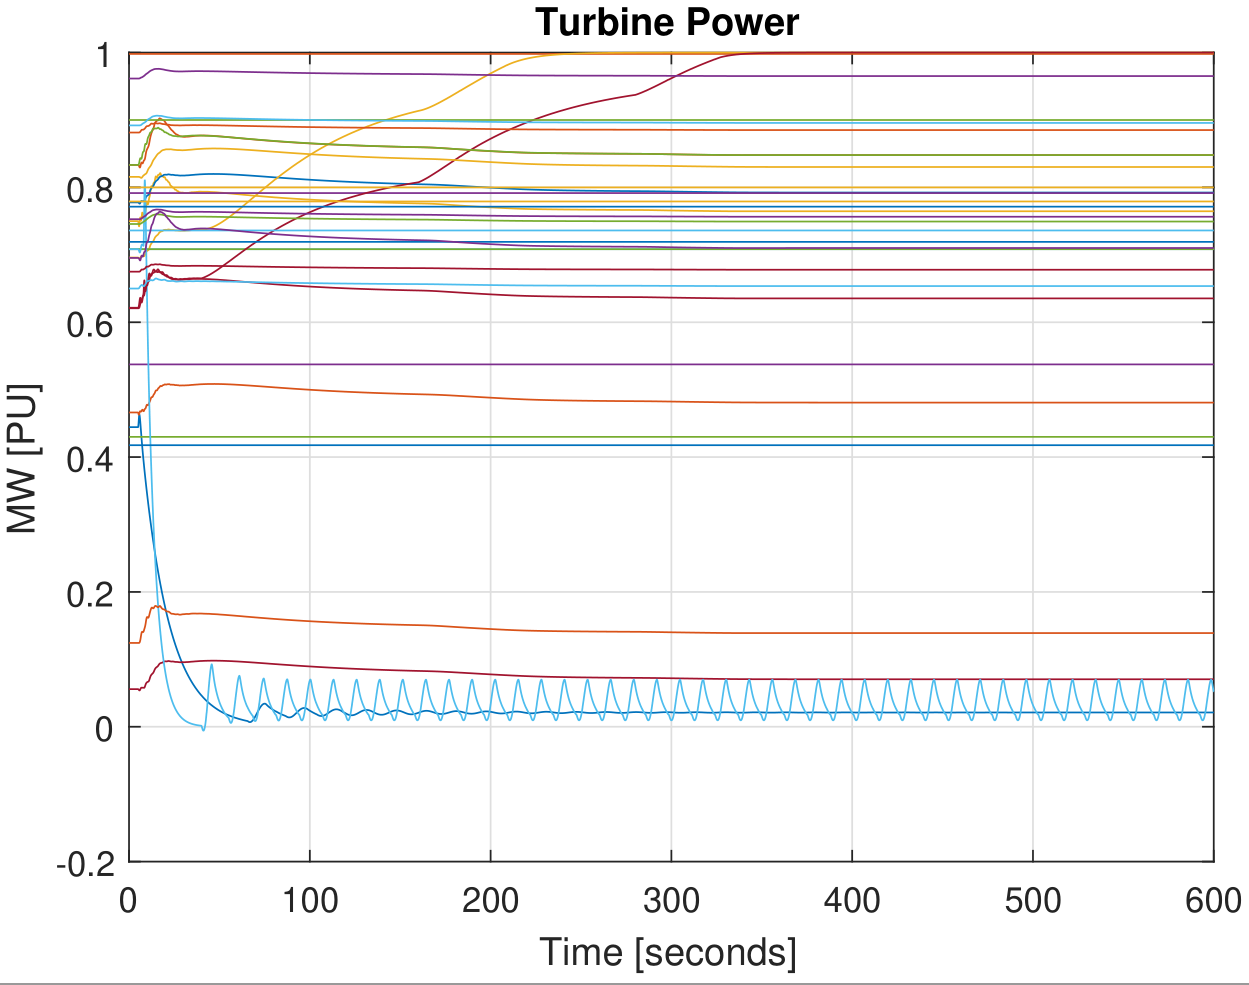
\includegraphics[width=.5\linewidth]{POW}
\end{center}

A possible solution may be to zero out the associated derivatives of tripped machines.

Something along the lines of:
\begin{minted}[
		frame=lines,
		framesep=2mm,
		baselinestretch=1.2,
		bgcolor=gray!13,
		fontsize=\footnotesize,
		%linenos,
		breaklines
		]{MATLAB}
if ~all(~g.mac.mac_trip_flags)
	g.mac.dXXX1 = g.mac.dXXX1 .* ~g.mac.mac_trip_flags
	g.mac.dXXX2 = g.mac.dXXX2 .* ~g.mac.mac_trip_flags
	...
end
\end{minted}

Placed in the \verb|handleStDx| function and called if the field is \verb|mac|.


This would prevent any associated states from changing, which may be confusing during data analysis and may have other network solution related effects, but should allow time step to increase.





\end{document}
